% ===== Page 81 =====
\subsection{Unitary Diagonalization}\label{ss:unitary}
\origpage{81}%
\begin{theorem}[Unitary diagonalization]
Let $A$ be an $n\times n$ Hermitian matrix. Then, \key{there exists a unitary matrix $P$} s.t.
\[
J = P\Hm A P .
\]
\end{theorem}
\begin{insight}[What $J$ looks like here]
For a Hermitian matrix the Jordan form $J$ is \emph{diagonal} with \emph{real} entries: the eigenvalues of $A=A\Hm$ are real, and $A$ is always diagonalizable (every eigenvalue has $m_j=1$ in the minimal polynomial). The theorem adds that the diagonalizing matrix can be chosen \emph{unitary}, i.e.\ $P^{-1}=P\Hm$, so that $A = PJP\Hm$ (unitary diagonalization).
\end{insight}
\begin{itemize}
\item[$\star$] \term{Unitary matrix}: $P^{-1} = P\Hm$.
\item[$\rightarrow$] \term{Orthogonal matrix} (real-valued unitary matrix): $P^{-1} = P\T$.
\item[$\star$] $P^{-1}P = PP^{-1} = I$, \quad i.e.\ \quad $P\Hm P = PP\Hm = I$.
\end{itemize}

\sep
\paragraph{Columns of a unitary matrix.}
\[
P = \bigl[\, p_1 \;\vdots\; p_2 \;\vdots\; \cdots \;\vdots\; p_n \,\bigr],
\qquad
P\Hm = \bmat{p_1\Hm\\ p_2\Hm\\ \vdots\\ p_n\Hm}
\]
\begin{align*}
P\Hm P &= \bmat{p_1\Hm\\ p_2\Hm\\ \vdots\\ p_n\Hm}\bigl[\, p_1 \;\vdots\; p_2 \;\vdots\; \cdots \;\vdots\; p_n \,\bigr]
= \bmat{p_1\Hm p_1 & p_1\Hm p_2 & \cdots & p_1\Hm p_n\\
p_2\Hm p_1 & p_2\Hm p_2 & \cdots & p_2\Hm p_n\\
\vdots & & & \vdots\\
p_n\Hm p_1 & & & p_n\Hm p_n}\\
&= \bmat{\inner{p_1}{p_1} & \inner{p_2}{p_1} & \cdots & \inner{p_n}{p_1}\\
\inner{p_1}{p_2} & & & \vdots\\
\vdots & & & \\
\inner{p_1}{p_n} & & & \inner{p_n}{p_n}}
\end{align*}
\explain{All entries are inner products, similar to a Gram matrix.}
$\Rightarrow$ \key{Columns of $P$ are orthonormal!}
\[
\inner{p_i}{p_j} = \delta_{ij} = \begin{cases} 1, & i=j\\ 0, & i\neq j\end{cases}
\]

% ===== Page 82 =====
\origpage{82}
\paragraph{Rows of a unitary matrix.}
\begingroup\renewcommand{\arraystretch}{1.25}%
\[
P = \bmat{r_1\\ \hline r_2\\ \hline \vdots\\ \hline r_n},
\qquad
\underbrace{\bmat{r_1\\ r_2\\ \vdots\\ r_n}}_{P}
\underbrace{\bigl[\, r_1\Hm \;\vdots\; r_2\Hm \;\vdots\; \cdots \;\vdots\; r_n\Hm \,\bigr]}_{P\Hm} = I
\]\endgroup
$\Rightarrow$ \key{Rows are also orthonormal!}

\begin{proof}[Proof (kind of proof, not an actual one)]
$A$ is Hermitian, $A\in\C^{5\times 5}$; $\lambda_1,\lambda_2$ are eigenvalues of $A$, $\lambda_1\neq\lambda_2$, and $\Sigma_j = A-\lambda_jI$:
\begin{align*}
d(s) &= (s-\lambda_1)^2(s-\lambda_2)^3\\
m(s) &= (s-\lambda_1)(s-\lambda_2)
\end{align*}
\[
\C^5 = \underbrace{\Null(\Sigma_1)}_{\dim 2} \overset{\perp}{\oplus} \underbrace{\Null(\Sigma_2)}_{\dim 3}
\]
\begin{center}
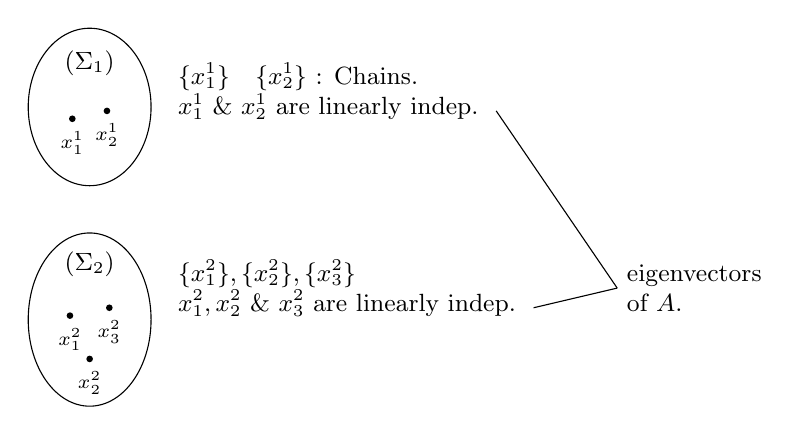
\begin{tikzpicture}[font=\small]
% ellipse N(Sigma_1)
\draw (0,0) ellipse (0.78 and 1.0);
\node at (0,0.55) {$\Null(\Sigma_1)$};
\fill (-0.22,-0.15) circle (1.2pt) node[below=1pt] {\scriptsize $x_1^1$};
\fill (0.22,-0.05) circle (1.2pt) node[below=1pt] {\scriptsize $x_2^1$};
\node[right,align=left] (t1) at (1.0,0.2) {$\{x_1^1\}\quad\{x_2^1\}$ : Chains.\\ $x_1^1$ \& $x_2^1$ are linearly indep.};
% ellipse N(Sigma_2)
\draw (0,-2.7) ellipse (0.78 and 1.1);
\node at (0,-2.0) {$\Null(\Sigma_2)$};
\fill (-0.25,-2.65) circle (1.2pt) node[below=1pt] {\scriptsize $x_1^2$};
\fill (0.25,-2.55) circle (1.2pt) node[below=1pt] {\scriptsize $x_3^2$};
\fill (0,-3.2) circle (1.2pt) node[below=1pt] {\scriptsize $x_2^2$};
\node[right,align=left] (t2) at (1.0,-2.3) {$\{x_1^2\},\{x_2^2\},\{x_3^2\}$\\ $x_1^2, x_2^2$ \& $x_3^2$ are linearly indep.};
% "eigenvectors of A" bracket
\draw (t1.east) ++(0.1,-0.25) -- (6.7,-2.3) coordinate (k);
\draw (t2.east) ++(0.1,-0.25) -- (k);
\node[right,align=left] at (k) {eigenvectors\\ of $A$.};
\end{tikzpicture}
\end{center}
\[
J = \bmat{\lambda_1 & & & & \\ & \lambda_1 & & \text{\Large 0} & \\ & & \lambda_2 & & \\ & \text{\Large 0} & & \lambda_2 & \\ & & & & \lambda_2}
\]
\[
P = \bigl[\, x_1^1 \;\vdots\; x_2^1 \;\vdots\; x_1^2 \;\vdots\; x_2^2 \;\vdots\; x_3^2 \,\bigr]_{5\times 5}
\]
$P$ is not directly unitary. The theorem states that there exists a unitary matrix $P$, which can be found. How can we convert $P$ to a unitary one?
\[
\underbrace{x_1^1\quad x_2^1}\qquad \underbrace{x_1^2\quad x_2^2\quad x_3^2}
\]
\explain{Vectors are orthogonal between the two sets. Vectors inside the sets are not necessarily orthogonal.}
\begin{insight}[Why eigenvectors of different eigenvalues are orthogonal]
If $Ax=\lambda_1x$, $Ay=\lambda_2y$ with $A=A\Hm$ (so $\lambda_1,\lambda_2\in\R$), then
\[
\lambda_1\, y\Hm x = y\Hm A x = (A y)\Hm x = \lambda_2\, y\Hm x
\ \Rightarrow\ (\lambda_1-\lambda_2)\,y\Hm x = 0
\ \Rightarrow\ y\Hm x = 0 .
\]
Gram--Schmidt inside each eigenspace keeps the vectors in that eigenspace (they remain eigenvectors), so the orthonormalized set still diagonalizes $A$.
\end{insight}
$\star$ We can apply \key{Gram--Schmidt orthonormalization to the two basis sets} and obtain the unitary matrix
\[
P = \bigl[\, e_1^1 \;\vdots\; e_2^1 \;\vdots\; e_1^2 \;\vdots\; e_2^2 \;\vdots\; e_3^2 \,\bigr].
\]
\end{proof}

% ===== Page 83 =====
\subsection{Spectral Decomposition}\label{ss:spectral-decomp}
\origpage{83}%
With $J = P\Hm A P$, we obtain the \term{spectral decomposition} of $A$:
\begingroup\renewcommand{\arraystretch}{1.25}%
\begin{align*}
A &= PJP\Hm\\
&= \bigl[\, e_1 \;\vdots\; e_2 \;\vdots\; \cdots \;\vdots\; e_n \,\bigr]
\bmat{\lambda_1 & & & \\ & \lambda_2 & & \\ & & \ddots & \\ & & & \lambda_n}
\bmat{e_1\Hm\\ \hline e_2\Hm\\ \hline \vdots\\ \hline e_n\Hm}\\
&= \bigl[\, \lambda_1 e_1 \;\vdots\; \lambda_2 e_2 \;\vdots\; \cdots \;\vdots\; \lambda_n e_n \,\bigr]
\bmat{e_1\Hm\\ \hline e_2\Hm\\ \hline \vdots\\ \hline e_n\Hm}\\
&= \lambda_1 e_1 e_1\Hm + \lambda_2 e_2 e_2\Hm + \cdots + \lambda_n e_n e_n\Hm\\[4pt]
&\boxed{A = \sum_{i=1}^{n} \lambda_i e_i e_i\Hm}
\end{align*}\endgroup
\begin{insight}
Each $e_ie_i\Hm$ is the orthogonal projection onto $\Span\{e_i\}$ (rank one, $(e_ie_i\Hm)^2=e_ie_i\Hm$). So a Hermitian matrix is a weighted sum of orthogonal projections onto its eigen-directions, weighted by the (real) eigenvalues. Also $\sum_i e_ie_i\Hm = PP\Hm = I$.
\end{insight}

\subsection{Positive Definite and Positive Semi-Definite Matrices}\label{ss:posdef}
\begin{definition}
A Hermitian matrix is said to be \term{positive definite} iff
\[
\inner{x}{Ax} > 0 \quad \forall x\neq 0 \qquad (x\Hm A x > 0).
\]
A Hermitian matrix is said to be \term{positive semi-definite} iff
\[
\inner{x}{Ax} \geq 0 \quad \forall x \qquad (x\Hm A x \geq 0).
\]
\end{definition}

\begin{theorem}
If a Hermitian matrix is positive definite, or positive semi-definite, then
\[
\underset{\text{(positive definite)}}{\lambda_i > 0} \quad\text{or}\quad \underset{\text{(positive semi-definite)}}{\lambda_i \geq 0} \quad\text{for all } i.
\]
\end{theorem}
\needspace{9\baselineskip}
\begin{proof}[Proof (only for the positive-definite case)]
Let $\lambda_i, e_i$ be an eigenpair, $e_i\neq 0$.
\begin{align*}
\inner{e_i}{Ae_i} &> 0\\
\inner{e_i}{\lambda_i e_i} &> 0\\
\lambda_i\inner{e_i}{e_i} &> 0\\
\lambda_i\norm{e_i}^2 &> 0
\end{align*}
\explain{$\norm{e_i}^2$ is positive (as $e_i\neq0$) $\Rightarrow$ $\lambda_i$ should be positive.}
% corrected: notes had "||e_i||^2 is non-negative"; strict positivity (e_i != 0) is what is needed
The semi-definite case is identical with ``$>$'' replaced by ``$\geq$''.
\end{proof}
\begin{insight}[Converse]
The converse also holds: with the spectral decomposition,
\[
x\Hm Ax = \sum_i \lambda_i\, x\Hm e_ie_i\Hm x = \sum_i\lambda_i\abs{e_i\Hm x}^2 .
\]
If all $\lambda_i>0$ this is $>0$ for $x\neq0$ (not all $e_i\Hm x$ vanish since $\{e_i\}$ is a basis). Hence \key{a Hermitian $A$ is positive definite $\iff$ all $\lambda_i>0$} (semi-definite $\iff$ all $\lambda_i\geq0$).
\end{insight}

% ===== Page 84 =====
\origpage{84}
\paragraph{Geometric interpretation.} $\star$ $\inner{x}{y} = \norm{x}\norm{y}\cdot\cos\theta$, so
\[
\inner{x}{Ax} = \underbrace{\norm{x}}_{>0}\;\underbrace{\norm{Ax}}_{>0}\;\cos\theta > 0 \quad \forall x\neq 0 .
\]
\explain{$\norm{Ax}>0$, otherwise the inner product would be 0.}
\explain{$\cos\theta>0$ $\hookrightarrow$ $-90^\circ < \theta < 90^\circ$.}
\begin{center}
\begin{tikzpicture}[scale=1.1]
\draw[->] (-1.7,0) -- (1.8,0);
\draw[->] (0,-1.5) -- (0,1.9);
\draw[->, thick] (0,0) -- (1.2,1.0) node[right] {$x$};
\draw[->, thick] (0,0) -- (-0.45,1.6);
% line through the origin perpendicular to x
\draw[dashed, gray] (-1.05,1.26) -- (0.9,-1.08);
\draw (0.154,0.128) -- ++(-0.128,0.154) -- ++(-0.154,-0.128);
\draw (0.38,0.32) arc (40:106:0.5);
\node at (0.2,0.85) {$\theta$};
\end{tikzpicture}
\end{center}

\section{Functions of a Matrix}\label{sec:functions}
\syllabusweek{Week 14 --- functions of a matrix}
\subsection{Definition via Power Series}\label{ss:fn-def}
\key{Functions of a matrix are \emph{not} applied entrywise}:
\begin{align*}
&\exp\!\left(\bmat{2&1\\1&2}\right) \neq \cancel{\bmat{e^2 & e\\ e & e^2}}
&& \text{MATLAB: } \cancel{\texttt{exp(A)}},\ \texttt{expm(A)}\ \checkmark\\
&\bmat{2&1\\1&2}^{1/2} \neq \cancel{\bmat{\sqrt2 & 1\\ 1 & \sqrt2}}
&& \text{MATLAB: } \cancel{\texttt{sqrt(A)}},\ \texttt{sqrtm(A)}\ \checkmark
\end{align*}
Motivation:
\[
\begin{array}{ll}
\dot{x} = Ax, & \dot{x} = ax,\\
x(t) = e^{At}x_0, & x(t) = e^{at}x_0,
\end{array}
\qquad
e^{At} = \sum_{i=0}^{\infty}\frac{(At)^i}{i!}.
\]

\sep
\paragraph{Taylor series.}
\[
f(s) = \sum_{i=0}^{\infty}\frac{f^{(i)}(s_0)}{i!}(s-s_0)^i,
\qquad
f^{(i)}(s_0) = \frac{d^i f}{ds^i}(s_0)
\]
% corrected: notes had d^i f / dt^i; the variable is s
If $s_0=0$:
\[
f(s) = \sum_{i=0}^{\infty}\underbrace{\frac{f^{(i)}(0)}{i!}}_{\alpha_i}\, s^i
\quad\Longrightarrow\quad
f(s) = \sum_{i=0}^{\infty}\alpha_i s^i
\]
For a matrix:
\begin{align*}
(\ast)\qquad f(A) &= \sum_{i=0}^{\infty}\frac{f^{(i)}(s_0)}{i!}(A-s_0I)^i\\
f(A) &= \sum_{i=0}^{\infty}\alpha_i A^i
\end{align*}

\sep
\paragraph{Reduction by Cayley--Hamilton.}
\begin{align*}
d(s) &= (s-\lambda_1)^{r_1}\cdots(s-\lambda_k)^{r_k}\\
d(s) &= s^n + d_1 s^{n-1} + \cdots + d_n\\
d(A) &= 0_{n\times n}\\
A^n &= -d_1A^{n-1} - d_2A^{n-2} - \cdots - d_nI
\end{align*}
Hence \key{all powers $A^i$, $i\geq n$, can be written using $I, A, \dots, A^{n-1}$}:
\[
f(A) = \sum_{i=0}^{\infty}\alpha_i A^i = c_0I + c_1A + c_2A^2 + \cdots + c_{n-1}A^{n-1}
\]
\explain{$c_0,c_1,\dots,c_{n-1}$: $n$ unknown coefficients.}

Using the minimal polynomial instead:\origpage{85}
\begin{align*}
m(s) &= (s-\lambda_1)^{m_1}\cdots(s-\lambda_k)^{m_k}, \qquad \ell = m_1 + m_2 + \cdots + m_k\\
m(s) &= s^\ell + g_1 s^{\ell-1} + \cdots + g_\ell, \qquad m(A) = 0_{n\times n}\\
% ===== Page 85 =====
A^\ell &= -g_1A^{\ell-1} - g_2A^{\ell-2} - \cdots - g_\ell I\\
f(A) &= c_0I + c_1A + \cdots + c_{\ell-1}A^{\ell-1}
\end{align*}
\explain{$c_0,c_1,\dots,c_{\ell-1}$: $\ell$ unknowns, $\ell\leq n$.}
\[
\left.\begin{aligned}
f(s) &= \sum_{i=0}^{\infty}\alpha_i s^i, & f(A) &= \sum_{i=0}^{\infty}\alpha_i A^i\\
p(s) &= \sum_{i=0}^{\ell-1}c_i s^i, & p(A) &= \sum_{i=0}^{\ell-1}c_i A^i
\end{aligned}\right\rangle
\ \boxed{f(A) = p(A)}\,.
\]
\needspace{7\baselineskip}
\begin{insight}[Why a polynomial of degree $\ell-1$ suffices]
Repeatedly substituting $A^\ell = -g_1A^{\ell-1}-\cdots-g_\ell I$ reduces every power $A^i$ ($i\geq\ell$) to a combination of $I,A,\dots,A^{\ell-1}$; summing the series gives $f(A)=\sum_{i=0}^{\ell-1}c_iA^i$. The coefficients $c_i$ depend on $f$ \emph{and} on $A$ (through $m(s)$), and the scalar polynomial $p(s)$ is in general \emph{not} equal to $f(s)$ --- only the matrix values agree. The next pages show that the $c_i$ are fixed by matching $f$ and $p$ (and derivatives) at the eigenvalues.
\end{insight}

Two methods to find $f(A)$:
\begin{itemize}[nosep]
\item \textbf{Method I:} Interpolating polynomial
\item \textbf{Method II:} Jordan canonical form
\end{itemize}

\subsection{Method I: Interpolating Polynomial (Diagonalizable Case)}\label{ss:method1-diag}
\paragraph{Case I: $A$ is diagonalizable.} Then $m(s) = (s-\lambda_1)(s-\lambda_2)\cdots(s-\lambda_k)$, \ $\ell = k$:
\[
p(s) = \sum_{i=0}^{\ell-1}c_i s^i, \qquad \ell = k \text{ is the \# of unknowns.}
\]
Let $\lambda_j, e_j$ be the eigenpairs, $j = 1,2,\dots,k$. First note
\begin{align*}
A^0 e_j &= \lambda_j^0 e_j = Ie_j\\
A e_j &= \lambda_j e_j\\
A^2 e_j &= A(Ae_j) = A\lambda_j e_j = \lambda_j Ae_j = \lambda_j^2 e_j\\
A^i e_j &= \lambda_j^i e_j
\end{align*}
Then
\begin{align*}
f(A)e_j &= p(A)e_j\\
\sum_{i=0}^{\infty}\alpha_i A^i e_j &= \sum_{i=0}^{\ell-1}c_i A^i e_j\\
\Bigl(\sum_{i=0}^{\infty}\alpha_i\lambda_j^i\Bigr)e_j &= \Bigl(\sum_{i=0}^{\ell-1}c_i\lambda_j^i\Bigr)e_j\\
f(\lambda_j)e_j &= p(\lambda_j)e_j\\
f(\lambda_j)e_j - p(\lambda_j)e_j &= 0
\end{align*}
\explain{$e_j$ is a nonzero vector.}
\[
\boxed{f(\lambda_j) = p(\lambda_j)}, \qquad j = 1,2,\dots,k
\]
$\Rightarrow$ \key{$k$ equations and $k$ unknowns}; we can solve these.

\begin{center}
\begin{minipage}{0.44\textwidth}
\centering
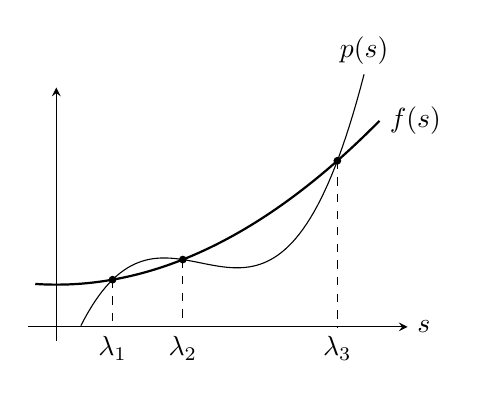
\begin{tikzpicture}
\begin{axis}[width=6.4cm,height=4.8cm,axis lines=middle,
  xmin=-0.4,xmax=5,ymin=-0.2,ymax=3.4,ticks=none,
  xlabel={$s$},xlabel style={anchor=west},clip=false]
\addplot[thick,domain=-0.3:4.6,samples=60] {0.6+0.11*x^2} node[right] {$f(s)$};
\addplot[domain=0.35:4.38,samples=80] {0.6+0.11*x^2+0.25*(x-0.8)*(x-1.8)*(x-4)} node[above] {$p(s)$};
\fill (axis cs:0.8,0.6704) circle (1.4pt);
\draw[dashed] (axis cs:0.8,0.6704) -- (axis cs:0.8,0) node[below] {$\lambda_1$};
\fill (axis cs:1.8,0.9564) circle (1.4pt);
\draw[dashed] (axis cs:1.8,0.9564) -- (axis cs:1.8,0) node[below] {$\lambda_2$};
\fill (axis cs:4,2.3600) circle (1.4pt);
\draw[dashed] (axis cs:4,2.3600) -- (axis cs:4,0) node[below] {$\lambda_3$};
\end{axis}
\end{tikzpicture}
\end{minipage}\hfill
\begin{minipage}{0.52\textwidth}
Although $p(s)$ \& $f(s)$ are different, they have the same values at the eigenvalues. Thus $p(s)$ is called the \term{interpolating polynomial}.
\[
\left.\begin{aligned} f(s) &\neq p(s)\\ f(A) &= p(A)\end{aligned}\right\rangle
\ \text{\small satisfied only at eigenvalues}
\]
\end{minipage}
\end{center}

% ===== Page 86 =====
\origpage{86}
\needspace{10\baselineskip}
\sep
\[
\underbrace{f(A)\cdot e_j}_{\text{matrix}\times\text{vector}} = \underbrace{f(\lambda_j)\,e_j}_{\text{scalar}\times\text{vector}}
\quad\Leftarrow\quad A\cdot e_j = \lambda_j e_j
\]
\explain{The eigenvalue is modified by the function $f$.}
\[
\begin{array}{lll} e^A & e^{\lambda_j} & e_j\\ \log A & \log\lambda_j & e_j \end{array}
\]
\explain{\key{Eigenvectors are invariant under functions}: $f(A)$ has the same eigenvectors $e_j$ as $A$, with eigenvalues $f(\lambda_j)$.}
% corrected: notes had "eigenvalues invariant under functions"; the eigenvectors e_j are what stays the same (eigenvalues become f(lambda_j))

\begin{example}
\[
A = \bmat{2&1\\1&2} \Rightarrow \lambda_1 = 3, \quad \lambda_2 = 1, \qquad
e_1 = \bmat{1\\1}, \quad e_2 = \bmat{1\\-1}
\]
\explain{Bunları nasıl buluyorduk? (How did we find these?) \ $Ae_1 = \lambda_1 e_1$, \ $[A-\lambda_1 I]e_1 = 0$.}
% note: "Bunlari nasil buluyorduk?" (Turkish) = "How did we find these?"
\explain{$d(s)=(s-2)^2-1=(s-3)(s-1)$; \ $A-3I=\left[\begin{smallmatrix}-1&1\\1&-1\end{smallmatrix}\right]\Rightarrow e_1=\left[\begin{smallmatrix}1\\1\end{smallmatrix}\right]$, \ $A-I=\left[\begin{smallmatrix}1&1\\1&1\end{smallmatrix}\right]\Rightarrow e_2=\left[\begin{smallmatrix}1\\-1\end{smallmatrix}\right]$.}
\begin{align*}
m(s) &= (s-3)(s-1)\\
\ell &= 2\\
p(s) &= c_0 + c_1 s
\end{align*}
Find $e^A$ \& $\log A$.

\paragraph{$e^A$.} $f(s) = e^s$; \ from $f(A) = p(A)$: \ $f(\lambda_j) = p(\lambda_j)$, \ $j = 1,2$:
\begin{align*}
f(3) &= e^3 = p(3) = c_0 + 3c_1\\
f(1) &= e = p(1) = c_0 + c_1\\[6pt]
\bmat{1&3\\1&1}\bmat{c_0\\c_1} &= \bmat{e^3\\e}\\
\Rightarrow\ \bmat{c_0\\c_1} &= -\frac12\bmat{1&-3\\-1&1}\bmat{e^3\\e}
= -\frac12\bmat{e^3-3e\\-e^3+e}\\
\Rightarrow\ c_0 &= \frac{3e-e^3}{2}, \qquad c_1 = \frac{e^3-e}{2}
\end{align*}
\explain{$\det\left[\begin{smallmatrix}1&3\\1&1\end{smallmatrix}\right]=-2$, so the inverse is $-\frac12\left[\begin{smallmatrix}1&-3\\-1&1\end{smallmatrix}\right]$.}
\[
\boxed{e^A = c_0I + c_1A = \frac{3e-e^3}{2}\bmat{1&0\\0&1} + \frac{e^3-e}{2}\bmat{2&1\\1&2}}
= \frac12\bmat{e^3+e & e^3-e\\ e^3-e & e^3+e}
\]
\begin{insight}[Check]
\[
e^A e_1 = \frac12\bmat{2e^3\\2e^3}=e^3e_1, \qquad e^Ae_2=\frac12\bmat{2e\\-2e}=e\,e_2,
\]
as required by $f(A)e_j=f(\lambda_j)e_j$. Numerically
\[
e^A\approx\bmat{11.402 & 8.684\\ 8.684 & 11.402},
\]
which agrees with summing the series $\sum_i A^i/i!$ (MATLAB \texttt{expm(A)}), while the entrywise $\left[\begin{smallmatrix}e^2&e\\e&e^2\end{smallmatrix}\right]$ is different.
\end{insight}

\paragraph{$\log A$.} $f(s) = \log s$, \ $f(\lambda_j) = p(\lambda_j)$, \ $j = 1,2$:
\begin{align*}
\log 3 &= c_0 + 3c_1\\
\log 1 &= c_0 + c_1 = 0 \ \Rightarrow\ c_0 = -c_1 \\ % corrected: notes had "log 0"; the eigenvalue is 1 and log 1 = 0
\log 3 &= 2c_1 \ \Rightarrow\ c_1 = \frac{\log 3}{2}, \qquad c_0 = -\frac{\log 3}{2} % corrected: notes had "c_2"; c_0 is meant
\end{align*}
\explain{Subtracting the second equation from the first gives $\log 3 = 2c_1$.}
\[
\boxed{\log A = -\frac{\log 3}{2}\bmat{1&0\\0&1} + \frac{\log 3}{2}\bmat{2&1\\1&2}}
= \frac{\log 3}{2}\bmat{1&1\\1&1}
\]
% corrected: notes had left-hand side "log s"; log A is meant
\explain{Check: $\log A\,e_1 = \log 3\; e_1$, \ $\log A\,e_2 = 0 = \log 1\; e_2$; and $e^{\log A}=A$.}

\paragraph{$e^{At}$.} $f(s) = e^{st}$, \ $f(\lambda_j) = p(\lambda_j)$, \ $j = 1,2$:
% corrected: written like f'(lambda_j) in the notes; f(lambda_j) is meant
\begin{align*}
e^{3t} &= c_0 + 3c_1 = c_0(t) + 3c_1(t)\\
e^{t} &= c_0 + c_1 = c_0(t) + c_1(t)
\end{align*}
\explain{Same linear system as for $e^A$ with $e^3\to e^{3t}$, $e\to e^t$; the coefficients now depend on $t$.}
\[
c_0(t) = \frac{3e^t - e^{3t}}{2}, \qquad c_1(t) = \frac{e^{3t}-e^t}{2}
\]
\[
\boxed{e^{At} = \frac{3e^t-e^{3t}}{2}\bmat{1&0\\0&1} + \frac{e^{3t}-e^t}{2}\bmat{2&1\\1&2}}
= \frac12\bmat{e^{3t}+e^t & e^{3t}-e^t\\ e^{3t}-e^t & e^{3t}+e^t}
\]
This solves
\[
\dot{x} = \bmat{2&1\\1&2}x,\quad x(0)=x_0
\qquad\Rightarrow\qquad x(t) = e^{At}x_0 .
\]
% corrected: notes had "x-dot = [2 1; 1 2] x_0"; the ODE is x-dot = A x with x(0) = x_0
\explain{Check: at $t=0$, $e^{A\cdot0}=I$; and $\frac{d}{dt}e^{At} = Ae^{At}$ (e.g.\ $(1,1)$ entry: $\frac{3e^{3t}+e^t}{2} = 2\cdot\frac{e^{3t}+e^t}{2}+\frac{e^{3t}-e^t}{2}$).}
\end{example}

% ===== Page 87 =====
\subsection{Method I: Non-Diagonalizable and General Case}\label{ss:method1-general}
\origpage{87}%
\paragraph{Case II: $A$ is not diagonalizable.}

\begin{example}
Let us have $A\in\R^{3\times3}$ and
\begin{align*}
m(s) &= (s-\lambda_1)^2(s-\lambda_2)\\
d(s) &= (s-\lambda_1)^2(s-\lambda_2) \qquad\text{as } A\in\R^{3\times3}
\end{align*}
\[
J = \left[\begin{array}{cc|c} \lambda_1 & 1 & 0\\ 0 & \lambda_1 & 0\\ \hline 0 & 0 & \lambda_2\end{array}\right],
\qquad
\underbrace{\Null(A-\lambda_1I)}_{1} \subsetneq \underbrace{\Null(A-\lambda_1I)^2}_{2} = \Null(A-\lambda_1I)^3
\]

\begin{center}
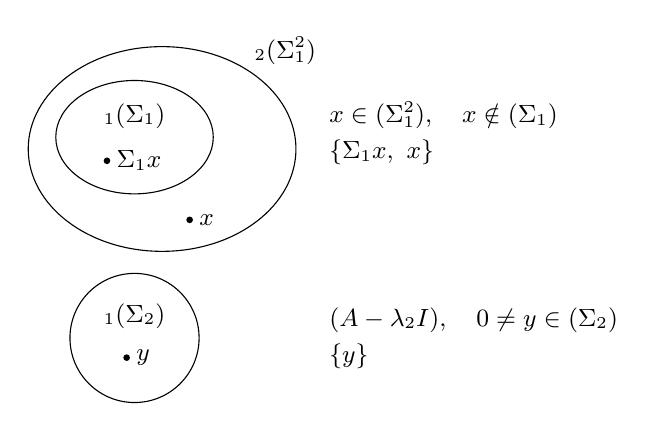
\begin{tikzpicture}[font=\small]
% nested null spaces of Sigma_1
\draw (0,0) ellipse (1.7 and 1.3);
\draw (-0.35,0.15) ellipse (1.0 and 0.72);
\node at (-0.35,0.42) {$\Null_1(\Sigma_1)$};
\fill (-0.7,-0.15) circle (1.2pt) node[right] {$\Sigma_1 x$};
\node[above right] at (1.05,0.95) {$\Null_2(\Sigma_1^2)$};
\fill (0.35,-0.9) circle (1.2pt) node[right] {$x$};
\node[right,align=left] at (2.0,0.2) {$x\in\Null(\Sigma_1^2),\quad x\notin\Null(\Sigma_1)$\\[2pt] $\{\Sigma_1x,\ x\}$};
% null space of Sigma_2
\draw (-0.35,-2.4) circle (0.82);
\node at (-0.35,-2.12) {$\Null_1(\Sigma_2)$};
\fill (-0.45,-2.65) circle (1.2pt) node[right] {$y$};
\node[right,align=left] at (2.0,-2.4) {$\Null(A-\lambda_2I),\quad 0\neq y\in\Null(\Sigma_2)$\\[2pt] $\{y\}$};
\end{tikzpicture}
\end{center}
\[
P = [\,\Sigma_1x \;\vdots\; x \;\vdots\; y\,] = [\,e_1 \;\vdots\; f_1 \;\vdots\; e_2\,],
\qquad f(A) = p(A)
\]
\begin{align*}
f(A)e_1 &= p(A)e_1\\
f(\lambda_1) &= p(\lambda_1)\\
f(\lambda_2) &= p(\lambda_2)
\end{align*}
\[
\ell = 3, \qquad \boxed{p(s) = c_0 + c_1s + c_2s^2}
\]
\explain{2 equations, but $c_0,c_1,c_2$: 3 unknowns $\Rightarrow$ we need one more.}
Use the generalized eigenvector $f_1$:
\[
f(A)\cdot f_1 = p(A)\cdot f_1,
\qquad
\sum_{i=0}^{\infty}\alpha_i A^i f_1 = \sum_{i=0}^{\ell-1}c_iA^if_1
\]
\begin{align*}
A^0 f_1 &= \lambda_1^0 f_1\\
Af_1 &= {?}
\end{align*}
\[
\Sigma_1 f_1 = e_1, \qquad (A-\lambda_1I)f_1 = e_1
\]
\[
\boxed{Af_1 = \lambda_1 f_1 + e_1}
\]
\explain{As $f_1$ is not an eigenvector, $Af_1$ should include $e_1$.}
\origpage{88}% (page 88 starts at the A^3 f_1 line)
\needspace{9\baselineskip}
\begin{align*}
A^2f_1 = A\cdot(Af_1) &= A(\lambda_1f_1 + e_1)\\
&= \lambda_1Af_1 + Ae_1\\
&= \lambda_1(\lambda_1f_1 + e_1) + \lambda_1e_1\\
&= \lambda_1^2f_1 + 2\lambda_1e_1\\
% ===== Page 88 =====
A^3f_1 = A(A^2f_1) &= A(\lambda_1^2f_1 + 2\lambda_1e_1)\\
&= \lambda_1^2(\lambda_1f_1+e_1) + 2\lambda_1^2e_1\\
&= \lambda_1^3f_1 + 3\lambda_1^2e_1
\end{align*}
\[
\boxed{A^2f_1 = \lambda_1^2 f_1 + 2\lambda_1 e_1}
\qquad
\boxed{A^3f_1 = \lambda_1^3f_1 + 3\lambda_1^2e_1}
\qquad
\boxed{A^if_1 = \lambda_1^if_1 + i\lambda_1^{i-1}e_1}
\]
Recall
\[
p(s) = \sum_{i=0}^{\ell-1}c_is^i, \qquad f(s) = \sum_{i=0}^{\infty}\alpha_is^i, \qquad f(\lambda_1) = p(\lambda_1), \qquad f(\lambda_2) = p(\lambda_2).
\]
Then
\begin{align*}
\Bigl(\sum_{i=0}^{\infty}\alpha_i\lambda_1^i\Bigr)f_1 + \Bigl(\sum_{i=0}^{\infty}\alpha_i\, i\lambda_1^{i-1}\Bigr)e_1
&= \Bigl(\sum_{i=0}^{\ell-1}c_i\lambda_1^i\Bigr)f_1 + \Bigl(\sum_{i=0}^{\ell-1}c_i\, i\lambda_1^{i-1}\Bigr)e_1\\
\cancel{f(\lambda_1)f_1} + f'(\lambda_1)e_1 &= \cancel{p(\lambda_1)f_1} + p'(\lambda_1)e_1
\end{align*}
\[
\boxed{f'(\lambda_1) = p'(\lambda_1)}
\]

\begin{minipage}[t]{0.45\textwidth}
3 equations:
\begin{align*}
p(\lambda_1) &= f(\lambda_1)\\
p(\lambda_2) &= f(\lambda_2)\\
p'(\lambda_1) &= f'(\lambda_1)
\end{align*}
\end{minipage}\hfill
\begin{minipage}[t]{0.5\textwidth}
If $m(s) = (s-\lambda_1)^3(s-\lambda_2)$:
\begin{align*}
p(\lambda_1) &= f(\lambda_1), & p(\lambda_2) &= f(\lambda_2)\\
p'(\lambda_1) &= f'(\lambda_1) & &\\
p''(\lambda_1) &= f''(\lambda_1) & &
\end{align*}
\end{minipage}
% note: the notes write only "p'  f'" and "p''  f''" in the last two rows
\end{example}

\subsubsection{General Case}
\[
m(s) = (s-\lambda_1)^{m_1}(s-\lambda_2)^{m_2}\cdots(s-\lambda_k)^{m_k}
\]
\[
\underbrace{c_0,c_1,\dots,c_{\ell-1}}_{\ell\text{ unknowns}}, \qquad \ell = m_1 + m_2 + \cdots + m_k
\]
\begin{keybox}
\[
f^{(t)}(\lambda_j) = p^{(t)}(\lambda_j), \qquad
t = 0,\dots,m_j-1 \ \ (m_j \text{ equations}), \quad j = 1,\dots,k
\]
\end{keybox}

\begin{example}
Find $\sin(\pi A)$ in terms of $A$, where
\[
A = \left[\begin{array}{ccc|cc|cc}
0&1&0 & & & & \\
0&0&1 & & & & \\
0&0&0 & & & & \\ \hline
 & & & 0&1 & & \\
 & & & 0&0 & & \\ \hline
 & & & & & 1&1\\
 & & & & & 0&1
\end{array}\right].
\]
\needspace{5\baselineskip}
\begin{align*}
d(s) &= (s-1)^2 s^5\\
m(s) &= (s-1)^2 s^3, \qquad \ell = 5\\
p(s) &= c_0 + c_1s + c_2s^2 + c_3s^3 + c_4s^4 \qquad (4^{\text{th}}\text{ order})
\end{align*}
Conditions and derivatives:
\[
\begin{array}{ll}
\bullet\ f(0) = p(0) & \bullet\ f(1) = p(1)\\
\bullet\ f'(0) = p'(0) & \bullet\ f'(1) = p'(1)\\
\bullet\ f''(0) = p''(0) &
\end{array}
\qquad\qquad
\begin{aligned}
f(s) &= \sin(\pi s)\\
f'(s) &= \pi\cos(\pi s)\\
f''(s) &= -\pi^2\sin(\pi s)
\end{aligned}
\]
% ===== Page 89 =====
\origpage{89}
\needspace{9\baselineskip}
\[
p'(s) = c_1 + 2c_2s + 3c_3s^2 + 4c_4s^3, \qquad
p''(s) = 2c_2 + 6c_3s + 12c_4s^2
\]
\begin{align*}
0 &= f(0) = p(0) = c_0\\
\pi &= f'(0) = p'(0) = c_1\\
0 &= f''(0) = p''(0) = 2c_2\\
0 &= f(1) = p(1) = c_1 + \cancel{c_2} + c_3 + c_4 + \cancel{c_0} = \pi + c_3 + c_4\\
-\pi &= f'(1) = p'(1) = c_1 + \cancel{2c_2} + 3c_3 + 4c_4 = \pi + 3c_3 + 4c_4
\end{align*}
% corrected: pass-2 transcription had c_1 struck through in p(1); c_1 = pi is not zero, it is substituted (giving c_3 + c_4 = -pi)
\explain{$f(0)=\sin0=0$, $f'(0)=\pi\cos0=\pi$, $f''(0)=-\pi^2\sin0=0$, $f(1)=\sin\pi=0$, $f'(1)=\pi\cos\pi=-\pi$.}
\[
\boxed{\begin{aligned} c_0 &= 0\\ c_1 &= \pi\\ c_2 &= 0\end{aligned}}
\quad\Rightarrow\quad
\begin{aligned} c_3 + c_4 &= -\pi\\ 3c_3 + 4c_4 &= -2\pi\end{aligned}
\quad\Rightarrow\quad
\boxed{\begin{aligned} c_3 &= -2\pi\\ c_4 &= \pi\end{aligned}}
\]
\[
\boxed{\sin(\pi A) = \pi A - 2\pi A^3 + \pi A^4}
\]
We still need to take 3$^{\text{rd}}$ (and 4$^{\text{th}}$) powers of $A$. If $A$ is in JCF, Method II will be much more efficient.
\begin{insight}[Check]
From $c_3+c_4=-\pi$: $c_4=-\pi-c_3$, so $3c_3-4\pi-4c_3=-2\pi \Rightarrow c_3=-2\pi$, $c_4=\pi$. Evaluating $\pi A-2\pi A^3+\pi A^4$ blockwise: for the nilpotent blocks $N$ ($3\times3$ and $2\times2$) $N^3=0$, so the result is $\pi N$; for the block $\left[\begin{smallmatrix}1&1\\0&1\end{smallmatrix}\right]$ it gives $\left[\begin{smallmatrix}0&-\pi\\0&0\end{smallmatrix}\right]$. This matches Method II below:
\[
\sin(\pi N)=\pi N-\frac{\pi^3}{6}N^3+\dots=\pi N,
\qquad
\sin\left(\pi\bmat{1&1\\0&1}\right)=\bmat{\sin\pi & \pi\cos\pi\\ 0&\sin\pi}=\bmat{0&-\pi\\0&0}.
\]
\end{insight}
\end{example}

\sep
\[
f^{(t)}(\lambda_j), \qquad t = 0,\dots,m_j-1, \quad j = 1,\dots,k
\]
If any derivative does not exist ($\infty$ or div 0), then \key{$f(A)$ does not exist}.

\begin{remark}
$f(A)$ does not exist when one of the $f^{(t)}(\lambda_j)$, $j = 1,2,\dots,k$; $t = 0,\dots,m_j-1$ does not exist.
% corrected: notes had f^{(t)}(A_j); lambda_j is meant
\end{remark}

\begin{example}
\[
A = \bmat{0&0\\0&1}, \qquad \lambda_1 = 0, \quad \lambda_2 = 1
\]
\begin{itemize}
\item $\cancel{\log A = {?}}$, \ $\cancel{\log s}$: gives infinity (at $\lambda_1=0$).
\item $\cancel{(I-A)^{-1} = {?}}$, \ $\cancel{(1-s)^{-1} = \tfrac{1}{1-s}}$ $\Rightarrow$ for $\lambda_2 = 1$: $\tfrac{1}{0} = \infty$.
\item $A^{-1}$ $\Longrightarrow$ function of a matrix. $s^{-1} = \dfrac1s$ $\Rightarrow$ if one of the eigenvalues is zero, the inverse does not exist.
\end{itemize}
\end{example}

\begin{example}
$f(s) = s^{1/2} = \sqrt{s}$, \qquad $A = \bmat{0&1\\0&0}$, \qquad $m(s) = s^2$.
\begin{align*}
&f(0) = p(0) && \Rightarrow\ \text{no problem}\\
&\cancel{f'(0) = p'(0)} && \Rightarrow\ \text{problem:}\quad
f'(s) = \frac{1}{2\sqrt s} \to \infty \text{ at } s = 0
\end{align*}
\explain{The square root function does not apply here: its derivative is not defined at the eigenvalue $s=0$.}
% corrected: notes had "Square root function DNA."; read as "does not apply" (f'(0) does not exist), consistent with the remark above
$\Rightarrow$ $\sqrt{A}$ does not exist for $A=\left[\begin{smallmatrix}0&1\\0&0\end{smallmatrix}\right]$.
\begin{insight}[Direct confirmation]
Suppose $X^2=A$ with $A=\left[\begin{smallmatrix}0&1\\0&0\end{smallmatrix}\right]$. Then $X^4=A^2=0$, so $X$ is nilpotent; a nilpotent $2\times2$ matrix satisfies $X^2=0$ (its minimal polynomial divides $s^2$). Hence $A=X^2=0$, a contradiction. So \emph{no} matrix squares to this $A$. In contrast, the zero matrix $\left[\begin{smallmatrix}0&0\\0&0\end{smallmatrix}\right]$ (with $m(s)=s$, only $f(0)$ needed) has the square root $0$: whether $f(A)$ exists depends on which derivatives the minimal polynomial requires, not only on the eigenvalues.
\end{insight}
\end{example}

% ===== Page 90 =====
\subsection{Method II: Jordan Canonical Form}\label{ss:method2}
\origpage{90}%
\[
J = \underbrace{P^{-1}AP}_{\substack{\text{similarity}\\ \text{transformation}}},
\qquad J \text{ is similar to } A.
\]
\key{Similar matrices have the same characteristic polynomial}:
\begin{align*}
B &= P^{-1}AP \qquad \bigl(\text{scalar analogue: } b = \cancel{p^{-1}}a\cancel{p} = a\bigr)\\
d_B(s) &= \det(sI-B) = \det(sI - P^{-1}AP)\\
&= \det\bigl(P^{-1}(sI-A)P\bigr) = \underbrace{\cancel{\det(P^{-1})}}_{\frac{1}{\det P}}\cdot\det(sI-A)\cdot\cancel{\det(P)}\\
d_B(s) &= d_A(s)
\end{align*}

\sep
Powers of $A = PJP^{-1}$:
\begin{align*}
(PJP^{-1})^0 &= I = PP^{-1} = P\cdot J^0P^{-1}\\
(PJP^{-1})^1 &= PJP^{-1}\\
(PJP^{-1})^2 &= PJ\cancel{P^{-1}}\cancel{P}JP^{-1} = PJ^2P^{-1}\\
(PJP^{-1})^i &= PJ^iP^{-1}
\end{align*}
\needspace{9\baselineskip}
Hence
\begin{align*}
f(A) &= \sum_{i=0}^{\infty}\alpha_i(PJP^{-1})^i = \sum_{i=0}^{\infty}\alpha_iP(J^i)P^{-1}\\
&= P\cdot\underbrace{\Bigl(\sum_{i=0}^{\infty}\alpha_iJ^i\Bigr)}_{f(J)}P^{-1}
\end{align*}
\[
\boxed{f(A) = Pf(J)P^{-1}}
\]

\sep
\paragraph{Block structure.}
\[
J = \bmat{J_1 & & & \\ & J_2 & & \\ & & \ddots & \\ & & & J_\sigma},
\qquad
J_t = \bmat{\lambda_j & 1 & & & \text{\Large 0}\\ & \lambda_j & 1 & & \\ & & \lambda_j & \ddots & \\ & & & \ddots & 1\\ \text{\Large 0} & & & & \lambda_j}_{d_t\times d_t}
\]
\explain{$J_t$ ($t=1,\dots,\sigma$) denotes a generic Jordan block of size $d_t$ belonging to the eigenvalue $\lambda_j$.}
% corrected: notes labelled the generic block J_sigma (size d_t) and the last block of J^i as J_t^i; made consistent (blocks J_1..J_sigma, generic block J_t)
\[
J^i = \bmat{J_1^i & & & \\ & J_2^i & & \\ & & \ddots & \\ & & & J_\sigma^i},
\qquad
f(J) = \sum_{i=0}^{\infty}\alpha_iJ^i = \bmat{\sum_{i=0}^{\infty}\alpha_iJ_1^i & & & \text{\Large 0}\\ & \sum_{i=0}^{\infty}\alpha_iJ_2^i & & \\ & & \ddots & \\ \text{\Large 0} & & & \sum_{i=0}^{\infty}\alpha_iJ_\sigma^i}
\]
\[
f(J) = \bmat{f(J_1) & & & \text{\Large 0}\\ & f(J_2) & & \\ & & \ddots & \\ \text{\Large 0} & & & f(J_\sigma)}
\]

\paragraph{One Jordan block.} Expanding around $s_0 = \lambda_j$ (advantageous):
\[
f(J_t) = \sum_{i=0}^{\infty}\alpha_iJ_t^i \underset{s_0 = \lambda_j}{=} \sum_{i=0}^{\infty}\frac{f^{(i)}(\lambda_j)}{i!}(J_t-\lambda_jI)^i
\]
\[
J_t - \lambda_jI = \bmat{0 & 1 & & \\ & 0 & \ddots & \\ & & \ddots & 1\\ & & & 0}_{d_t\times d_t},
\qquad
(J_t-\lambda_jI)^2 = \bmat{0 & 0 & 1 & & \\ & \ddots & \ddots & \ddots & \\ & & \ddots & \ddots & 1\\ & & & \ddots & 0\\ & & & & 0}_{d_t\times d_t}
\]
\explain{Each power shifts the line of 1's one diagonal up ($\nearrow$).}

% ===== Page 91 =====
\origpage{91}
\[
(\ast)\qquad (J_t-\lambda_jI)^d = 0, \qquad d\geq d_t
\]
\[
(J_t-\lambda_jI)^{d_t-1} = \bmat{ & & 0 & 1\\ & \text{\Large 0} & & 0\\ & & & \\ & & & },
\qquad
(J_t-\lambda_jI)^0 = \bmat{1 & & \text{\Large 0}\\ & \ddots & \\ \text{\Large 0} & & 1}
\]
\[
f(J_t) = \sum_{i=0}^{d_t-1}\frac{f^{(i)}(\lambda_j)}{i!}(J_t-\lambda_jI)^i
\]
\explain{Upper limit $d_t-1$ due to $(\ast)$.}
\begin{keybox}
\[
f(J_t) = \bmat{
f(\lambda_j) & f'(\lambda_j) & \frac{f''(\lambda_j)}{2!} & \cdots & \frac{f^{(d_t-1)}(\lambda_j)}{(d_t-1)!}\\
 & f(\lambda_j) & f'(\lambda_j) & \frac{f''(\lambda_j)}{2!} & \vdots\\
 & & \ddots & \ddots & \frac{f''(\lambda_j)}{2!}\\
 & \text{\huge 0} & & \ddots & f'(\lambda_j)\\
 & & & & f(\lambda_j)}
\]
\end{keybox}
\begin{itemize}[nosep]
\item The $0^{\text{th}}$ power ($I$) forms the main diagonal.
\item The $1^{\text{st}}$ power forms the first superdiagonal.
\item[] \quad $\vdots$
\end{itemize}
\begin{insight}[Link with Method I]
$f(J_t)$ only uses $f(\lambda_j),f'(\lambda_j),\dots,f^{(d_t-1)}(\lambda_j)$. The largest block of $\lambda_j$ has size $m_j$ (the exponent in $m(s)$), so Methods I and II use exactly the same data $f^{(t)}(\lambda_j)$, $t=0,\dots,m_j-1$; in particular $f(A)$ exists iff these derivatives exist. Method II avoids solving for $c_0,\dots,c_{\ell-1}$ and computing powers of $A$, but needs $P$ and $P^{-1}$.
\end{insight}

\begin{example}
\[
A = \bmat{2&1\\1&2}, \qquad
\lambda_1 = 3,\ \lambda_2 = 1,
\qquad e_1 = \bmat{1\\1}, \quad e_2 = \bmat{1\\-1}
\]
\[
P = [\,e_1 \;\vdots\; e_2\,], \qquad A = P\underbrace{\left[\begin{array}{c|c}3&0\\ \hline 0&1\end{array}\right]}_{J}P^{-1}
\qquad\Rightarrow\qquad
f(A) = P\left[\begin{array}{c|c} f(3) & 0\\ \hline 0 & f(1)\end{array}\right]P^{-1}
\]
With $P=\left[\begin{smallmatrix}1&1\\1&-1\end{smallmatrix}\right]$ and $P^{-1}=\frac12\left[\begin{smallmatrix}1&1\\1&-1\end{smallmatrix}\right]$:
\[
f(A) = \frac12\bmat{f(3)+f(1) & f(3)-f(1)\\ f(3)-f(1) & f(3)+f(1)} .
\]
\explain{For $f(s)=e^s$, $\log s$, $e^{st}$ this reproduces the Method I results $e^A$, $\log A$, $e^{At}$ above.}
\end{example}

\begin{example}
Find $\sin(\pi A)$ for
\[
A = \left[\begin{array}{ccc|cc|c}
\frac12 & 1 & 0 & & & \\
0 & \frac12 & 1 & & & \\
0 & 0 & \frac12 & & & \\ \hline
 & & & \frac32 & 1 & \\
 & & & 0 & \frac32 & \\ \hline
 & & & & & \frac52
\end{array}\right]
= \bmat{J_1 & & \\ & J_2 & \\ & & J_3}.
\]
\begin{align*}
&A = PJP^{-1}, \quad P = I \text{ chosen} \Rightarrow A = J\\
&d(s) = \left(s-\tfrac12\right)^3\left(s-\tfrac32\right)^2\left(s-\tfrac52\right)\\
&m(s) = \left(s-\tfrac12\right)^3\left(s-\tfrac32\right)^2\left(s-\tfrac52\right)^1\\
&p(s) = c_0 + c_1s + c_2s^2 + c_3s^3 + c_4s^4 + c_5s^5
\end{align*}
\explain{Method I $\hookrightarrow$ too complicated; use Method II blockwise.}

% ===== Page 92 =====
\origpage{92}
\[
f(s) = \sin(\pi s), \qquad f'(s) = \pi\cos(\pi s), \qquad f''(s) = -\pi^2\sin(\pi s)
\]
\[
\sin(\pi J_1) = \bmat{1 & 0 & -\frac{\pi^2}{2}\\ 0 & 1 & 0\\ 0 & 0 & 1},
\qquad
\sin(\pi J_2) = \bmat{-1 & 0\\ 0 & -1},
\qquad
\sin(\pi J_3) = \bmat{1}
\]
\explain{$J_1$ ($\lambda=\tfrac12$, size 3): $f(\tfrac12)=1$, \ $f'(\tfrac12)=\pi\cos\tfrac{\pi}{2}=0$, \ $f''(\tfrac12)/2!=-\pi^2/2$.}
\explain{$J_2$ ($\lambda=\tfrac32$, size 2): $f(\tfrac32)=-1$, \ $f'(\tfrac32)=\pi\cos\tfrac{3\pi}{2}=0$.}
\explain{$J_3$ ($\lambda=\tfrac52$, size 1): $f(\tfrac52)=\sin\tfrac{5\pi}{2}=1$.}
\[
\sin(\pi A) = \left[\begin{array}{ccc|cc|c}
1 & 0 & -\frac{\pi^2}{2} & & & \\
0 & 1 & 0 & & & \\
0 & 0 & 1 & & & \\ \hline
 & & & -1 & 0 & \\
 & & & 0 & -1 & \\ \hline
 & & & & & 1
\end{array}\right]
\]
\end{example}

\begin{example}[Square root of a matrix]
\[
f(s) = \sqrt{s} = s^{1/2},
\qquad
A = \bmat{2&1\\1&2},
\qquad
A^{1/2} = P\bmat{\sqrt3 & 0\\ 0 & \sqrt1}P^{-1} \ \Rightarrow\ \text{unique}
\]
\explain{$\hookrightarrow$ unique positive-definite square root of $A$: MATLAB $\cancel{\texttt{sqrt(A)}}$, \ $\texttt{sqrtm(A)}\ \checkmark$.}
But if we only require $A^{1/2}\cdot A^{1/2} = A$ $\Rightarrow$ not unique anymore (compare: $x = \sqrt3$ vs.\ $y\cdot y = 3$):
\begin{align*}
A^{1/2}\cdot A^{1/2} &= P\bmat{3&0\\0&1}P^{-1}\\
A^{1/2} &= P\bmat{-\sqrt3 & 0\\ 0 & \sqrt1}P^{-1} \ \Rightarrow\ A^{1/2}A^{1/2} = P\bmat{3&0\\0&1}P^{-1}\\
A^{1/2} &= P\bmat{\pm\sqrt3 & 0\\ 0 & \pm\sqrt1}P^{-1}
\end{align*}
% corrected: notes had \mp in both entries; the two signs can be chosen independently (4 matrices)
\explain{These are all valid for the definition $A^{1/2}A^{1/2} = A$ (signs chosen independently: 4 matrices).}
\begin{insight}[The numbers]
With $P=\left[\begin{smallmatrix}1&1\\1&-1\end{smallmatrix}\right]$,
\[
P\diag(a,b)P^{-1}=\frac12\bmat{a+b&a-b\\a-b&a+b},
\qquad
\bigl(P\diag(a,b)P^{-1}\bigr)^2=\frac12\bmat{a^2+b^2&a^2-b^2\\a^2-b^2&a^2+b^2},
\]
which equals $A$ whenever $a^2=3$, $b^2=1$. The principal (function) square root is
\[
A^{1/2} = \text{\texttt{sqrtm(A)}} =\frac12\bmat{\sqrt3+1 & \sqrt3-1\\ \sqrt3-1 & \sqrt3+1}\approx\bmat{1.366&0.366\\0.366&1.366},
\]
whose eigenvalues $\sqrt3,1$ are positive: it is \key{the unique positive-definite square root}. The other three choices $(a,b)=(-\sqrt3,1),(\sqrt3,-1),(-\sqrt3,-1)$ also square to $A$ but are not positive definite.
\end{insight}
If $A$ is positive definite $\Rightarrow$ the square root is wanted to be positive definite, which is given by the function.
\end{example}
